% ============================================================================
% TOPIC 18C: TRANSITION-STATE THEORY
% ============================================================================

\section{Topic 18C: Transition-State Theory}

% ===========================================================================
% Slide 35: Topic 18C Overview
% ===========================================================================
\begin{frame}{Topic 18C: Overview}

\textbf{Transition-State Theory (TST) / Activated Complex Theory (ACT)}

\vspace{0.3cm}

\begin{itemize}
    \item The most sophisticated "classical" theory of reaction rates.
    \item Developed by Eyring, Evans, and Polanyi (1930s).
    \item \textbf{Key Concept:} Focus on the species at the top of the energy barrier.
\end{itemize}

\vspace{0.3cm}
\textbf{Goals:}
\begin{itemize}
    \item Calculate rates from thermodynamic properties ($\Delta G^\ddagger$, $\Delta H^\ddagger$, $\Delta S^\ddagger$).
    \item Explain kinetic salt effects.
    \item Explain kinetic isotope effects.
\end{itemize}

\end{frame}

% ===========================================================================
% Slide: The Reaction Coordinate
% ===========================================================================
\begin{frame}{The Reaction Coordinate}

\begin{columns}[T]
\column{0.5\textwidth}
\begin{itemize}
    \item \textbf{Reactants (A+B)}
    \item \textbf{Transition State ($\ddagger$)}: Point of maximum energy.
    \item \textbf{Activated Complex (C$^\ddagger$)}: The molecular species at the transition state.
    \item \textbf{Products (P)}
\end{itemize}

\column{0.5\textwidth}
\centering
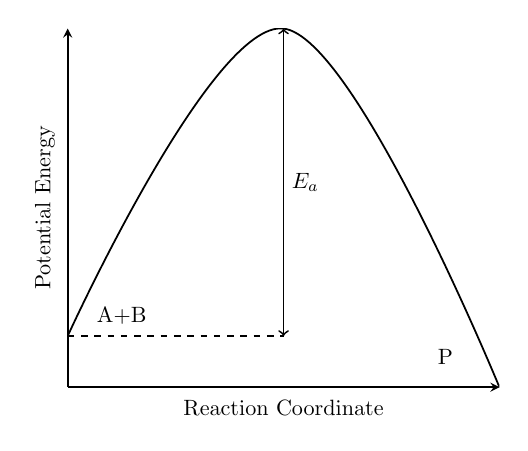
\begin{tikzpicture}[scale=0.8]
    \begin{axis}[
        xlabel={Reaction Coordinate},
        ylabel={Potential Energy},
        xtick=\empty, ytick=\empty,
        axis lines=left,
        thick
    ]
    \addplot[smooth, tension=0.6] coordinates {(0,1) (2,4) (4,0.5)};
    \node at (axis cs:0.5,1.2) {A+B};
    \node at (axis cs:2,4.3) {C$^\ddagger$};
    \node at (axis cs:3.5,0.8) {P};
    \draw[dashed] (axis cs:0,1) -- (axis cs:2,1);
    \draw[<->] (axis cs:2,1) -- (axis cs:2,4) node[midway, right] {$E_a$};
    \end{axis}
\end{tikzpicture}
\end{columns}

\end{frame}

% ===========================================================================
% Slide: Fundamental Assumptions of TST
% ===========================================================================
\begin{frame}{Fundamental Assumptions of TST}

\textbf{Three Key Assumptions:}

\begin{enumerate}
    \item \textbf{Quasi-Equilibrium:} The activated complex C$^\ddagger$ is in equilibrium with reactants.
    \[ \text{A} + \text{B} \underset{K^\ddagger}{\rightleftharpoons} \text{C}^\ddagger \]

    \item \textbf{Factorization:} The reaction coordinate motion can be separated from other degrees of freedom.

    \item \textbf{One-Way Crossing:} Once formed, C$^\ddagger$ always proceeds to products (transmission coefficient $\kappa \approx 1$).
\end{enumerate}

\vspace{0.3cm}
\textbf{Validity:} These assumptions work well when:
\begin{itemize}
    \item Barrier is high compared to $k_B T$
    \item No significant recrossing of barrier
    \item No quantum tunneling (for classical TST)
\end{itemize}

\end{frame}

% ===========================================================================
% Slide: The Big Idea
% ===========================================================================
\begin{frame}{The Big Idea}

\textbf{Fundamental Approach:}
The activated complex C$^\ddagger$ is in \alert{quasi-equilibrium} with the reactants.

\[ \text{A} + \text{B} \underset{K^\ddagger}{\rightleftharpoons} \text{C}^\ddagger \xrightarrow{k^\ddagger} \text{P} \]

\vspace{0.3cm}
The rate of reaction is:
\[ \text{Rate} = k^\ddagger [\text{C}^\ddagger] \]

\begin{itemize}
    \item $[\text{C}^\ddagger]$: Concentration of activated complex (from equilibrium).
    \item $k^\ddagger$: Frequency of crossing the barrier.
\end{itemize}

\vspace{0.3cm}
\textbf{Strategy:}
\begin{enumerate}
    \item Calculate $[\text{C}^\ddagger]$ from equilibrium thermodynamics
    \item Calculate $k^\ddagger$ from the reaction coordinate vibration frequency
    \item Combine to get the rate constant
\end{enumerate}

\end{frame}

% ===========================================================================
% Slide: Statistical Mechanics Foundation
% ===========================================================================
\begin{frame}{Statistical Mechanics Foundation}

\textbf{Partition Functions:}

For a molecular species $i$, the molecular partition function is:
\[ q_i = \sum_j g_j e^{-\varepsilon_j/k_B T} \]

The equilibrium constant relates to partition functions:
\keyeq{K^\ddagger = \frac{[\text{C}^\ddagger]}{[\text{A}][\text{B}]} = \frac{q_{\text{C}^\ddagger}}{q_{\text{A}} q_{\text{B}}} \frac{N_A}{V} e^{-E_0/RT}}

where $E_0$ is the zero-point energy difference.

\vspace{0.3cm}
\textbf{Key Insight:} The partition function includes contributions from:
\begin{itemize}
    \item Translation: $q_{\text{trans}} \propto V T^{3/2} m^{3/2}$
    \item Rotation: $q_{\text{rot}} \propto T^{3/2}$ (nonlinear)
    \item Vibration: $q_{\text{vib}} = \prod_i \frac{1}{1-e^{-h\nu_i/k_B T}}$
\end{itemize}

\end{frame}

% ===========================================================================
% Slide: Factorization of Reaction Coordinate
% ===========================================================================
\begin{frame}{Factorization of Reaction Coordinate}

\textbf{Critical Step:} Separate the reaction coordinate from $q_{\text{C}^\ddagger}$

The transition state has one "loose" vibration along the reaction coordinate with frequency $\nu^\ddagger$.

For this mode:
\[ q_{\text{RC}} = \frac{1}{1-e^{-h\nu^\ddagger/k_B T}} \approx \frac{k_B T}{h\nu^\ddagger} \quad \text{(classical limit)} \]

Therefore:
\keyeq{q_{\text{C}^\ddagger} = \left(\frac{k_B T}{h\nu^\ddagger}\right) \bar{q}_{\text{C}^\ddagger}}

where $\bar{q}_{\text{C}^\ddagger}$ is the partition function with the reaction coordinate removed.

\end{frame}

% ===========================================================================
% Slide: Rate of Decay - Vibrational Motion
% ===========================================================================
\begin{frame}{Rate of Decay}

\textbf{How fast does C$^\ddagger$ fall apart into products?}

\begin{itemize}
    \item The motion along the reaction coordinate is a "loose vibration".
    \item Frequency of this vibration = $\nu^\ddagger$.
    \item Rate constant for crossing: $k^\ddagger = \kappa \nu^\ddagger$.
    \item $\kappa$: Transmission coefficient (usually $\approx 1$).
\end{itemize}

\vspace{0.3cm}
\textbf{Physical Picture:}
\begin{itemize}
    \item At the transition state, the molecule "vibrates" along the reaction path
    \item Each vibration has a chance to proceed to products
    \item For classical barrier crossing: every forward crossing leads to products ($\kappa = 1$)
    \item For tunneling or recrossing: $\kappa \neq 1$
\end{itemize}

\end{frame}

% ===========================================================================
% Slide: Derivation of Eyring Equation - Step 1
% ===========================================================================
\begin{frame}{Derivation of Eyring Equation - Step 1}

\textbf{Concentration of activated complex:}

From equilibrium:
\[ [\text{C}^\ddagger] = K^\ddagger [\text{A}][\text{B}] \]

Substituting partition functions:
\[ [\text{C}^\ddagger] = \frac{q_{\text{C}^\ddagger}}{q_{\text{A}} q_{\text{B}}} \frac{N_A}{V} e^{-E_0/RT} [\text{A}][\text{B}] \]

Factor out reaction coordinate:
\[ [\text{C}^\ddagger] = \frac{k_B T}{h\nu^\ddagger} \frac{\bar{q}_{\text{C}^\ddagger}}{q_{\text{A}} q_{\text{B}}} \frac{N_A}{V} e^{-E_0/RT} [\text{A}][\text{B}] \]

\end{frame}

% ===========================================================================
% Slide: Derivation of Eyring Equation - Step 2
% ===========================================================================
\begin{frame}{Derivation of Eyring Equation - Step 2}

\textbf{Rate of reaction:}

\[ \text{Rate} = \kappa \nu^\ddagger [\text{C}^\ddagger] \]

Substitute expression for $[\text{C}^\ddagger]$:
\[ \text{Rate} = \kappa \nu^\ddagger \times \frac{k_B T}{h\nu^\ddagger} \frac{\bar{q}_{\text{C}^\ddagger}}{q_{\text{A}} q_{\text{B}}} \frac{N_A}{V} e^{-E_0/RT} [\text{A}][\text{B}] \]

\alert{The frequency $\nu^\ddagger$ cancels!}

\[ \text{Rate} = \kappa \frac{k_B T}{h} \frac{\bar{q}_{\text{C}^\ddagger}}{q_{\text{A}} q_{\text{B}}} \frac{N_A}{V} e^{-E_0/RT} [\text{A}][\text{B}] \]

\end{frame}

% ===========================================================================
% Slide: The Eyring Equation - Final Form
% ===========================================================================
\begin{frame}{The Eyring Equation - Final Form}

\textbf{Rate constant:}

\keyeq{k_r = \kappa \frac{k_B T}{h} \bar{K}^\ddagger}

Or in thermodynamic terms:
\keyeq{k_r = \kappa \frac{k_B T}{h} e^{-\Delta^\ddagger G^\circ / RT}}

where $\Delta^\ddagger G^\circ$ is the standard Gibbs energy of activation.

\vspace{0.3cm}
\textbf{Key Features:}
\begin{itemize}
    \item Universal pre-factor: $\frac{k_B T}{h} \approx 6.2 \times 10^{12}$ s$^{-1}$ at 298 K
    \item Temperature dependence: $T e^{-\Delta^\ddagger H^\circ / RT}$ (not just exponential!)
    \item Connection to thermodynamics through $\Delta^\ddagger G^\circ$
\end{itemize}

\end{frame}

% ===========================================================================
% Slide: Eyring Equation - Physical Interpretation
% ===========================================================================
\begin{frame}{Eyring Equation - Interpretation}

\[ k_r = \frac{k_B T}{h} e^{-\Delta^\ddagger G^\circ / RT} \]

\begin{itemize}
    \item $\frac{k_B T}{h}$: \textbf{Universal Frequency Factor}.
    \begin{itemize}
        \item At 300 K, $\approx 6 \times 10^{12}$ s$^{-1}$.
        \item Sets the fundamental timescale of chemical reactions.
        \item Origin: Typical vibrational frequency at TS.
    \end{itemize}
    \item $\Delta^\ddagger G^\circ$: \textbf{Gibbs Energy of Activation}.
    \begin{itemize}
        \item Determines the barrier height.
        \item Includes both enthalpy and entropy contributions.
        \item Can be measured experimentally.
    \end{itemize}
\end{itemize}

\vspace{0.3cm}
\textbf{Maximum Rate:} If $\Delta^\ddagger G^\circ = 0$, then $k_r \approx 6 \times 10^{12}$ s$^{-1}$ - the \alert{diffusion-limited rate}.

\end{frame}

% ===========================================================================
% Slide: Thermodynamic Formulation
% ===========================================================================
\begin{frame}{Thermodynamic Formulation}

Expand $\Delta^\ddagger G^\circ = \Delta^\ddagger H^\circ - T\Delta^\ddagger S^\circ$:

\keyeq{k_r = \frac{k_B T}{h} e^{\Delta^\ddagger S^\circ / R} e^{-\Delta^\ddagger H^\circ / RT}}

\textbf{Comparison with Arrhenius ($k = A e^{-E_a/RT}$):}
\begin{itemize}
    \item \textbf{Enthalpy ($\Delta^\ddagger H^\circ$)} $\leftrightarrow$ Activation Energy ($E_a$).
    \item \textbf{Entropy ($\Delta^\ddagger S^\circ$)} $\leftrightarrow$ Pre-exponential Factor ($A$).
\end{itemize}

\vspace{0.3cm}
\textbf{Key Advantage:} TST separates:
\begin{itemize}
    \item Energetic barrier ($\Delta^\ddagger H^\circ$)
    \item Structural/entropic effects ($\Delta^\ddagger S^\circ$)
\end{itemize}

\end{frame}

% ===========================================================================
% Slide: Relating Parameters
% ===========================================================================
\begin{frame}{Relating TST to Arrhenius Parameters}

\textbf{Enthalpy vs. Activation Energy:}

Starting from definitions:
\[ E_a = RT^2 \frac{d \ln k}{dT} \]

For Eyring equation $k = \frac{k_B T}{h} e^{-\Delta^\ddagger G^\circ / RT}$:

\begin{itemize}
    \item \textbf{Solution:} $E_a = \Delta^\ddagger H^\circ + RT$
    \item \textbf{Gas Phase (bimolecular):} $E_a = \Delta^\ddagger H^\circ + 2RT$
    \item \textbf{Gas Phase (unimolecular):} $E_a = \Delta^\ddagger H^\circ + RT$
\end{itemize}

\vspace{0.3cm}
\textbf{Entropy vs. A-Factor:}
\[ A = \frac{e k_B T}{h} e^{\Delta^\ddagger S^\circ / R} \]

where $e = 2.718$ (Euler's number).

\end{frame}

% ===========================================================================
% Slide: Eyring Plot
% ===========================================================================
\begin{frame}{Eyring Plot}

\textbf{Linearization for experimental analysis:}

Take logarithm of $k = \frac{k_B T}{h} e^{\Delta^\ddagger S^\circ / R} e^{-\Delta^\ddagger H^\circ / RT}$:

\keyeq{\ln\left(\frac{k}{T}\right) = \ln\left(\frac{k_B}{h}\right) + \frac{\Delta^\ddagger S^\circ}{R} - \frac{\Delta^\ddagger H^\circ}{RT}}

\textbf{Plot:} $\ln(k/T)$ vs. $1/T$ gives straight line
\begin{itemize}
    \item \textbf{Slope:} $-\Delta^\ddagger H^\circ / R$
    \item \textbf{Intercept:} $\ln(k_B/h) + \Delta^\ddagger S^\circ/R$
\end{itemize}

\vspace{0.3cm}
\textbf{Advantage over Arrhenius:} Direct determination of $\Delta^\ddagger H^\circ$ and $\Delta^\ddagger S^\circ$.

\end{frame}

% ===========================================================================
% Slide: Activation Entropy Part 1
% ===========================================================================
\begin{frame}{Activation Entropy ($\Delta^\ddagger S^\circ$) - Part 1}

\textbf{Physical Meaning:}

\[ \Delta^\ddagger S^\circ = S^\circ_{\text{C}^\ddagger} - S^\circ_{\text{A}} - S^\circ_{\text{B}} \]

\vspace{0.3cm}

\textbf{Negative $\Delta^\ddagger S^\circ$ (Associative):}

Transition state is \textbf{more ordered} than reactants.

\begin{itemize}
    \item Example: Dimerization ($A + A \to A_2^\ddagger$)
    \item Two molecules coming together lose translational freedom
    \item Typically: $\Delta^\ddagger S^\circ \approx -100$ to $-150$ J/(mol·K)
\end{itemize}

\end{frame}

% ===========================================================================
% Slide: Activation Entropy Part 2
% ===========================================================================
\begin{frame}{Activation Entropy ($\Delta^\ddagger S^\circ$) - Part 2}

\textbf{Positive $\Delta^\ddagger S^\circ$ (Dissociative):}

Transition state is \textbf{more disordered} than reactants.

\begin{itemize}
    \item Example: Bond breaking in unimolecular decomposition
    \item Increased vibrational freedom
    \item Typically: $\Delta^\ddagger S^\circ > 0$
\end{itemize}

\vspace{0.3cm}

\textbf{Near-Zero $\Delta^\ddagger S^\circ$:}
\begin{itemize}
    \item Similar structure to reactants
    \item Minor reorganization at transition state
\end{itemize}

\vspace{0.3cm}

\emphbox{The sign of $\Delta^\ddagger S^\circ$ reveals the geometry of the transition state}

\end{frame}

% ===========================================================================
% Slide: Free Energy Diagrams
% ===========================================================================
\begin{frame}{Free Energy Diagrams}

\textbf{Effect of $\Delta^\ddagger S^\circ$ on reaction profile:}

\begin{center}
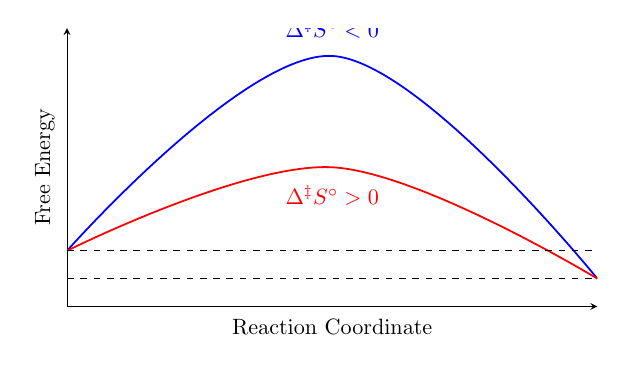
\begin{tikzpicture}[scale=0.8]
    \begin{axis}[
        xlabel={Reaction Coordinate},
        ylabel={Free Energy},
        xtick=\empty,
        ytick=\empty,
        axis lines=left,
        width=10cm,
        height=6cm,
        ymin=0, ymax=5
    ]
    % Negative entropy (higher barrier)
    \addplot[blue, thick, smooth, tension=0.6] coordinates {(0,1) (2,4.5) (4,0.5)};
    \node[blue] at (axis cs:2,5) {$\Delta^\ddagger S^\circ < 0$};

    % Positive entropy (lower barrier)
    \addplot[red, thick, smooth, tension=0.6] coordinates {(0,1) (2,2.5) (4,0.5)};
    \node[red] at (axis cs:2,2) {$\Delta^\ddagger S^\circ > 0$};

    \draw[dashed] (axis cs:0,1) -- (axis cs:4,1) node[right] {Reactants};
    \draw[dashed] (axis cs:0,0.5) -- (axis cs:4,0.5) node[right] {Products};
    \end{axis}
\end{tikzpicture}
\end{center}

At higher $T$: Negative $\Delta^\ddagger S^\circ$ becomes more unfavorable ($-T\Delta^\ddagger S^\circ$ increases).

\end{frame}

% ===========================================================================
% Slide: Hammond Postulate
% ===========================================================================
\begin{frame}{Hammond Postulate}

\textbf{Relating TS structure to thermodynamics:}

\vspace{0.3cm}
\emphbox{
\textbf{Hammond Postulate:} The structure of the transition state resembles the structure of the nearest stable species (reactant, product, or intermediate).
}

\vspace{0.3cm}
\textbf{Implications:}

\begin{columns}[T]
\column{0.5\textwidth}
\textbf{Endergonic Reaction:}
\begin{itemize}
    \item TS resembles products
    \item "Late" transition state
    \item Product-like structure
\end{itemize}

\column{0.5\textwidth}
\textbf{Exergonic Reaction:}
\begin{itemize}
    \item TS resembles reactants
    \item "Early" transition state
    \item Reactant-like structure
\end{itemize}
\end{columns}

\vspace{0.3cm}
\textbf{Application:} Helps predict effects of substituents on reaction rates.

\end{frame}

% ===========================================================================
% Slide: The Kinetic Salt Effect
% ===========================================================================
\begin{frame}{The Kinetic Salt Effect}

\textbf{For reactions between ions in solution:} $A^{z_A} + B^{z_B} \to C^\ddagger \to P$

\textbf{Debye-Hückel Theory predicts:}
\keyeq{\log(k_r) = \log(k_r^\circ) + 2A z_A z_B \sqrt{I}}

\begin{itemize}
    \item $I$: Ionic strength of solution = $\frac{1}{2}\sum_i c_i z_i^2$.
    \item $z_A, z_B$: Charges of reactants.
    \item $A$: Constant = 0.509 M$^{-1/2}$ for water at 25°C.
    \item $k_r^\circ$: Rate constant at zero ionic strength.
\end{itemize}

\vspace{0.3cm}
\textbf{Physical Origin:}
\begin{itemize}
    \item Ionic atmosphere screens charge interactions
    \item Affects activation energy for charged reactants
    \item Charge on TS: $z_\ddagger = z_A + z_B$
\end{itemize}

\end{frame}

% ===========================================================================
% Slide: Kinetic Salt Effect - Predictions Part 1
% ===========================================================================
\begin{frame}{Kinetic Salt Effect - Predictions (Part 1)}

\textbf{Effect of Ionic Strength on Rate:}

\vspace{0.3cm}

\textbf{Like charges ($z_A z_B > 0$):} Rate \alert{increases} with ionic strength.
\begin{itemize}
    \item Example: S$_2$O$_8^{2-}$ + I$^-$
    \item $z_A z_B = (-2)(-1) = +2 > 0$: rate increases
    \item Ionic atmosphere reduces repulsion
\end{itemize}

\vspace{0.3cm}

\textbf{Opposite charges ($z_A z_B < 0$):} Rate \alert{decreases} with ionic strength.
\begin{itemize}
    \item Example: [Co(NH$_3$)$_5$Br]$^{2+}$ + OH$^-$
    \item $z_A z_B = (+2)(-1) = -2 < 0$: rate decreases
    \item Ionic atmosphere screens attraction
\end{itemize}

\end{frame}

% ===========================================================================
% Slide: Kinetic Salt Effect - Predictions Part 2
% ===========================================================================
\begin{frame}{Kinetic Salt Effect - Predictions (Part 2)}

\begin{columns}[T]
\column{0.5\textwidth}
\textbf{Summary:}
\begin{itemize}
    \item $z_A z_B > 0$: rate increases with $I$
    \item $z_A z_B < 0$: rate decreases with $I$
    \item $z_A z_B = 0$: no primary salt effect
\end{itemize}

\column{0.5\textwidth}
\centering
\includegraphics[width=\textwidth]{Reaction_Dynamics_Interactive/images/kinetic_salt_effect.png}

\vspace{0.1cm}
\tiny \textit{Interactive calculator: See notebook at end}
\end{columns}

\vspace{0.3cm}

\emphbox{Slope of plot gives information about charges in the transition state}

\end{frame}

% ===========================================================================
% Slide: Kinetic Isotope Effects Part 1
% ===========================================================================
\begin{frame}{Kinetic Isotope Effects (KIE) - Part 1}

\textbf{What happens if we replace H with D (or $^{12}$C with $^{13}$C)?}

\vspace{0.3cm}

\textbf{Origin:} Zero-point energy (ZPE) difference.

\[ \text{ZPE} = \frac{1}{2}h\nu = \frac{1}{2}h\frac{1}{2\pi}\sqrt{\frac{k}{\mu}} \]

\vspace{0.3cm}

\textbf{Physical Effect:}
\begin{itemize}
    \item Heavier isotope has lower ZPE (smaller $\nu$)
    \item C-D bond is stronger than C-H bond by $\sim 5$ kJ/mol
    \item Requires more energy to break
    \item Reaction becomes slower
\end{itemize}

\vspace{0.3cm}

\keyeq{\frac{k_H}{k_D} \approx 7 \text{ (at 25}^\circ\text{C)}}

\end{frame}

% ===========================================================================
% Slide: Kinetic Isotope Effects Part 2
% ===========================================================================
\begin{frame}{Kinetic Isotope Effects (KIE) - Part 2}

\textbf{Types of KIE:}

\vspace{0.3cm}

\textbf{Primary KIE:} Bond to H/D breaks in rate-determining step
\begin{itemize}
    \item $k_H/k_D = 2$-$10$ (typical range)
    \item Large effect indicates bond breaking at TS
    \item Example: C-H bond cleavage in radical abstraction
\end{itemize}

\vspace{0.3cm}

\textbf{Secondary KIE:} Bond to H/D does not break
\begin{itemize}
    \item $k_H/k_D = 1.1$-$1.5$ (small effect)
    \item Due to hybridization changes at TS
    \item Example: Adjacent to reaction center
\end{itemize}

\vspace{0.3cm}

\emphbox{KIE is a powerful tool for identifying mechanisms and rate-determining steps}

\end{frame}

% ===========================================================================
% Slide: Zero-Point Energy Diagram
% ===========================================================================
\begin{frame}{Zero-Point Energy and KIE}

\begin{center}
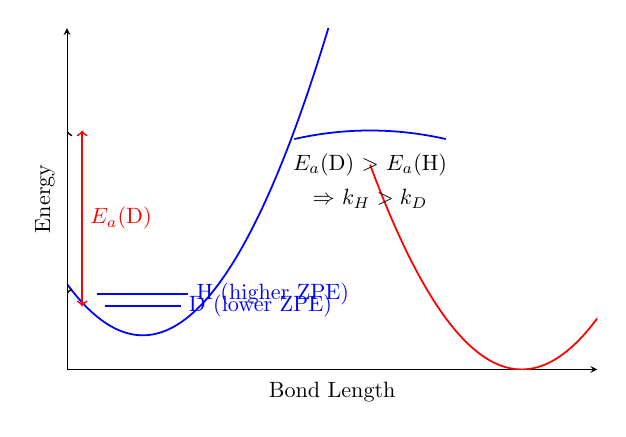
\begin{tikzpicture}[scale=0.8]
    \begin{axis}[
        xlabel={Bond Length},
        ylabel={Energy},
        xtick=\empty,
        ytick=\empty,
        axis lines=left,
        width=10cm,
        height=7cm,
        ymin=0, ymax=5
    ]
    % Reactant potential (same curvature = same force constant)
    \addplot[blue, thick, domain=0.5:2.5, samples=100] {3*(x-1)^2 + 0.5};
    % Barrier region
    \addplot[blue, thick, domain=2:3, samples=50] {3.5 - 0.5*(x-2.5)^2};
    % Product potential (same curvature as reactant)
    \addplot[red, thick, domain=2.5:4, samples=100] {3*(x-3.5)^2};

    % ZPE levels: ν ∝ √(k/m), so ZPE_D/ZPE_H = √(m_H/m_D) = 1/√2
    % Place H ZPE at 0.6 above minimum (0.5), so ZPE_H level at 1.1
    % D ZPE = 0.6/√2 = 0.424 above minimum, so level at 0.924
    \draw[blue, thick] (axis cs:0.7,1.1) -- (axis cs:1.3,1.1) node[right] {H (higher ZPE)};
    \draw[blue, thick] (axis cs:0.75,0.924) -- (axis cs:1.25,0.924) node[right] {D (lower ZPE)};

    % Activation energies (from ZPE levels to barrier top at ~3.5)
    \draw[<->, thick] (axis cs:0.5,1.1) -- (axis cs:0.5,3.5) node[midway, left] {$E_a$(H)};
    \draw[<->, thick, red] (axis cs:0.6,0.924) -- (axis cs:0.6,3.5) node[midway, right] {$E_a$(D)};

    \node at (axis cs:2.5,3) {$E_a$(D) $>$ $E_a$(H)};
    \node at (axis cs:2.5,2.5) {$\Rightarrow$ $k_{\text{H}} > k_{\text{D}}$};
    \end{axis}
\end{tikzpicture}
\end{center}

Difference in $E_a$: $\Delta E_a \approx \frac{1}{2}h(\nu_{\text{H}} - \nu_{\text{D}}) \approx 5$ kJ/mol

\end{frame}

% ===========================================================================
% Slide: Quantum Tunneling Part 1
% ===========================================================================
\begin{frame}{Quantum Tunneling (Part 1)}

\textbf{Classical TST assumes:} Over-the-barrier crossing.

\textbf{Quantum Reality:} Particles can pass \textit{through} the barrier!

\vspace{0.3cm}

\textbf{When is tunneling important?}
\begin{itemize}
    \item Significant for light particles (H$^+$, e$^-$)
    \item More important at low temperatures
    \item Pronounced for narrow, high barriers
\end{itemize}

\vspace{0.3cm}

\textbf{Experimental Evidence:}
\begin{itemize}
    \item $k_H/k_D \gg 7$ (e.g., 10-100, much larger than classical KIE)
    \item Curved Arrhenius plots (concave upward)
    \item Unusual temperature dependence (rate less sensitive to T)
\end{itemize}

\end{frame}

% ===========================================================================
% Slide: Quantum Tunneling Part 2
% ===========================================================================
\begin{frame}{Quantum Tunneling (Part 2)}

\begin{columns}[T]
\column{0.5\textwidth}
\textbf{Two Pathways:}

\vspace{0.2cm}

\textcolor{blue}{\textbf{Over:}} Classical barrier crossing

\textcolor{red}{\textbf{Through:}} Quantum tunneling

\vspace{0.3cm}

Tunneling bypasses the activation barrier!

\column{0.5\textwidth}
\centering
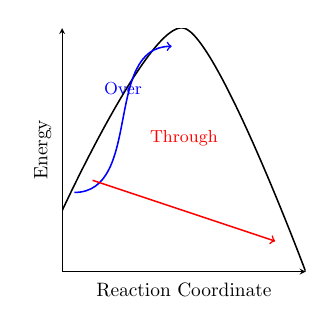
\begin{tikzpicture}[scale=0.7]
    \begin{axis}[
        xlabel={Reaction Coordinate},
        ylabel={Energy},
        xtick=\empty, ytick=\empty,
        axis lines=left,
        height=6cm,
        width=6cm
    ]
    \addplot[smooth, thick] coordinates {(0,0) (2,3) (4,-1)};
    \draw[blue, thick, ->] (0.2,0.3) to[out=0, in=180] (1.8,2.7);
    \node[blue] at (1,2) {\small Over};
    \draw[red, thick, ->] (0.5,0.5) -- (3.5,-0.5);
    \node[red] at (2,1.2) {\small Through};
    \end{axis}
\end{tikzpicture}
\end{columns}

\vspace{0.3cm}

\textbf{Bell's Correction:}
\[ \kappa = \frac{Q_{\text{tunnel}}}{Q_{\text{classical}}} = \frac{u/2}{\sin(u/2)}, \quad u = \frac{h\nu_{\text{barrier}}}{k_B T} \]

\end{frame}

% ===========================================================================
% Slide: Linear Free Energy Relationships (LFER)
% ===========================================================================
\begin{frame}{Linear Free Energy Relationships}

\textbf{Brønsted Catalysis Law:}

For acid-catalyzed reactions:
\keyeq{\log k = \log G + \alpha \log K_a}

where $K_a$ is the acidity constant.

\begin{itemize}
    \item $\alpha$: Brønsted coefficient ($0 \leq \alpha \leq 1$)
    \item Measures how much charge is transferred in TS
    \item $\alpha \approx 0$: TS resembles reactants (early TS)
    \item $\alpha \approx 1$: TS resembles products (late TS)
\end{itemize}

\vspace{0.3cm}
\textbf{Related Relationships:}
\begin{itemize}
    \item \textbf{Hammett equation:} For substituted benzene derivatives
    \item \textbf{Marcus relationship:} For electron transfer
    \item \textbf{Polanyi relationship:} $E_a = E_0 + \alpha \Delta H_{\text{rxn}}$
\end{itemize}

\end{frame}

% ===========================================================================
% Slide: Worked Example 1
% ===========================================================================
\begin{frame}{Worked Example 1: Calculating Rate Constant}

\textbf{Problem:} A reaction has $\Delta^\ddagger H^\circ = 85$ kJ/mol and $\Delta^\ddagger S^\circ = -45$ J/(mol·K). Calculate the rate constant at 298 K.

\vspace{0.3cm}
\textbf{Solution:}

Step 1: Calculate $\Delta^\ddagger G^\circ$
\[ \Delta^\ddagger G^\circ = \Delta^\ddagger H^\circ - T\Delta^\ddagger S^\circ \]
\[ = 85000 - 298 \times (-45) = 85000 + 13410 = 98410 \text{ J/mol} \]

Step 2: Apply Eyring equation
\[ k = \frac{k_B T}{h} e^{-\Delta^\ddagger G^\circ / RT} \]
\[ = \frac{1.381 \times 10^{-23} \times 298}{6.626 \times 10^{-34}} \times e^{-98410/(8.314 \times 298)} \]
\[ = 6.21 \times 10^{12} \times e^{-39.7} = 6.21 \times 10^{12} \times 7.84 \times 10^{-18} \]
\keyeq{k = 4.87 \times 10^{-5} \text{ s}^{-1}}

\end{frame}

% ===========================================================================
% Slide: Worked Example 2
% ===========================================================================
\begin{frame}{Worked Example 2: Activation Parameters from Data}

\textbf{Problem:} Rate constants measured at two temperatures:
\begin{itemize}
    \item $k(300 \text{ K}) = 1.5 \times 10^{-3}$ s$^{-1}$
    \item $k(320 \text{ K}) = 8.2 \times 10^{-3}$ s$^{-1}$
\end{itemize}
Calculate $\Delta^\ddagger H^\circ$ and $\Delta^\ddagger S^\circ$ (assume $\kappa = 1$).

\vspace{0.3cm}
\textbf{Solution:}

From Eyring plot: $\ln(k/T) = \ln(k_B/h) + \Delta^\ddagger S^\circ/R - \Delta^\ddagger H^\circ/(RT)$

Calculate slope:
\[ \text{slope} = \frac{\ln(k_2/T_2) - \ln(k_1/T_1)}{1/T_2 - 1/T_1} \]
\[ = \frac{\ln(8.2 \times 10^{-3}/320) - \ln(1.5 \times 10^{-3}/300)}{1/320 - 1/300} \]
\[ = \frac{-10.05 - (-10.72)}{-2.08 \times 10^{-4}} = \frac{0.67}{-2.08 \times 10^{-4}} = -3221 \text{ K} \]

Therefore: $\Delta^\ddagger H^\circ = -R \times \text{slope} = 8.314 \times 3221 = 26.8$ kJ/mol

\end{frame}

% ===========================================================================
% Slide: Worked Example 3
% ===========================================================================
\begin{frame}{Worked Example 3: Salt Effect}

\textbf{Problem:} For the reaction:
\[ \text{[Co(NH}_3\text{)}_5\text{Br]}^{2+} + \text{OH}^- \to \text{products} \]

The rate constant at zero ionic strength is $k_0 = 1.2 \times 10^{-4}$ M$^{-1}$s$^{-1}$. Predict the rate constant at $I = 0.05$ M.

\vspace{0.3cm}
\textbf{Solution:}

Charges: $z_A = +2$, $z_B = -1$, so $z_A z_B = -2$

Apply salt effect equation:
\[ \log(k) = \log(k_0) + 2A z_A z_B \sqrt{I} \]
\[ = \log(1.2 \times 10^{-4}) + 2(0.509)(-2)\sqrt{0.05} \]
\[ = -3.92 + 2(0.509)(-2)(0.224) = -3.92 - 0.456 = -4.38 \]

\keyeq{k = 10^{-4.38} = 4.2 \times 10^{-5} \text{ M}^{-1}\text{s}^{-1}}

The rate decreases by a factor of $\sim 3$ due to screening of attraction.

\end{frame}

% ===========================================================================
% Slide: Practice Problem 1
% ===========================================================================
\begin{frame}{Practice Problem 1}
\vspace{-0.2cm}
\textbf{Problem:} At 298 K: $\Delta^\ddagger H^\circ = 60$ kJ/mol, $\Delta^\ddagger S^\circ = -80$ J/(mol·K)

\vspace{0.15cm}
\begin{enumerate}[a),topsep=0pt,itemsep=1pt]
    \item Calculate $\Delta^\ddagger G^\circ$ at 298 K.
    \item Calculate the rate constant ($\kappa = 1$).
    \item Is TS more or less ordered?
    \item How does $k$ change at 350 K?
\end{enumerate}

\vspace{0.2cm}
\textbf{Answers:}
\begin{itemize}[topsep=0pt,itemsep=1pt]
    \item[(a)] $\Delta^\ddagger G^\circ = 83.8$ kJ/mol
    \item[(b)] $k = 9.8 \times 10^{-3}$ s$^{-1}$
    \item[(c)] More ordered ($\Delta^\ddagger S^\circ < 0$)
    \item[(d)] $k(350\text{ K}) = 0.51$ s$^{-1}$ (50$\times$ faster)
\end{itemize}

\end{frame}

% ===========================================================================
% Slide: Practice Problem 2
% ===========================================================================
\begin{frame}{Practice Problem 2}

\textbf{Problem:} The rate constant for H-abstraction by a radical is $k_{\text{H}} = 5.0 \times 10^6$ M$^{-1}$s$^{-1}$ at 298 K. The same reaction with deuterium has $k_{\text{D}} = 8.3 \times 10^5$ M$^{-1}$s$^{-1}$.

\begin{enumerate}[a)]
    \item Calculate the kinetic isotope effect $k_{\text{H}}/k_{\text{D}}$.
    \item Is this a primary or secondary KIE?
    \item What does this tell you about the mechanism?
    \item Estimate the difference in activation energies.
\end{enumerate}

\vspace{0.5cm}
\textbf{Answers:}
\begin{itemize}
    \item[(a)] KIE $= 6.0$
    \item[(b)] Primary KIE
    \item[(c)] C-H bond breaking occurs in rate-determining step
    \item[(d)] $\Delta E_a \approx 4.4$ kJ/mol (from $\ln(6.0) = \Delta E_a/(RT)$)
\end{itemize}

\end{frame}

% ===========================================================================
% Slide: Practice Problem 3
% ===========================================================================
\begin{frame}{Practice Problem 3}
\vspace{-0.2cm}
\textbf{Problem:} For an ionic reaction:

\begin{center}
\small
\begin{tabular}{cc}
$\sqrt{I}$ (M$^{1/2}$) & $k$ (M$^{-1}$s$^{-1}$) \\
\hline
0 & $2.0 \times 10^{-3}$ \\
0.1 & $3.2 \times 10^{-3}$ \\
0.2 & $5.1 \times 10^{-3}$ \\
\end{tabular}
\end{center}

\vspace{0.1cm}
\begin{enumerate}[a),topsep=0pt,itemsep=1pt]
    \item Plot $\log k$ vs $\sqrt{I}$ and find slope.
    \item Determine $z_A z_B$.
    \item Like or opposite charge?
\end{enumerate}

\vspace{0.15cm}
\textbf{Answers:}
\begin{itemize}[topsep=0pt,itemsep=1pt]
    \item[(a)] Slope $\approx 2.0$
    \item[(b)] From slope $= 2A z_A z_B$: $z_A z_B = +2$
    \item[(c)] Like charges
\end{itemize}

\end{frame}

% ===========================================================================
% Slide: Practice Problem 4
% ===========================================================================
\begin{frame}{Practice Problem 4}

\textbf{Problem:} An Eyring plot gives:
\begin{itemize}
    \item Slope $= -8500$ K
    \item Intercept $= 25.5$
\end{itemize}

Calculate $\Delta^\ddagger H^\circ$ and $\Delta^\ddagger S^\circ$.

\vspace{0.5cm}
\textbf{Solution:}

From slope:
\[ \Delta^\ddagger H^\circ = -R \times \text{slope} = 8.314 \times 8500 = 70.7 \text{ kJ/mol} \]

From intercept:
\[ \text{intercept} = \ln(k_B/h) + \Delta^\ddagger S^\circ/R \]
\[ 25.5 = 23.76 + \Delta^\ddagger S^\circ/8.314 \]
\[ \Delta^\ddagger S^\circ = (25.5 - 23.76) \times 8.314 = 14.5 \text{ J/(mol·K)} \]

\textbf{Answer:} $\Delta^\ddagger H^\circ = 70.7$ kJ/mol, $\Delta^\ddagger S^\circ = +14.5$ J/(mol·K)

Positive entropy suggests a dissociative transition state.

\end{frame}

% ===========================================================================
% Slide: Summary Topic 18C
% ===========================================================================
\begin{frame}{Summary: Topic 18C}

\begin{enumerate}
    \item \textbf{Eyring Equation:} Links rates to thermodynamics through $\Delta^\ddagger G^\circ$.
    \[ k = \frac{k_B T}{h} e^{-\Delta^\ddagger G^\circ / RT} \]

    \item \textbf{Activation Parameters:}
        \begin{itemize}
            \item $\Delta^\ddagger H^\circ \approx E_a - RT$ (solution)
            \item $\Delta^\ddagger S^\circ$ reflects structure of transition state
        \end{itemize}

    \item \textbf{Salt Effects:} Ionic strength affects rates between ions.
    \[ \log(k) = \log(k_0) + 2A z_A z_B \sqrt{I} \]

    \item \textbf{Isotope Effects:} Probe bond breaking and tunneling.
    \item \textbf{LFER:} Connect structure to reactivity (Brønsted, Hammett).
\end{enumerate}

\end{frame}

% ===========================================================================
% Slide: Interactive Resources for Topic 18C
% ===========================================================================
\begin{frame}{Interactive Learning: Topic 18C}

\begin{columns}[c]
\column{0.65\textwidth}
\textbf{Explore Transition-State Theory Interactively!}

\vspace{0.3cm}

\textbf{Interactive Jupyter Notebook Features:}
\begin{itemize}
    \item \textbf{Eyring Plot Generator}: Calculate $\Delta^\ddagger H^\circ$ and $\Delta^\ddagger S^\circ$
    \item \textbf{KIE Calculator}: Explore kinetic isotope effects
    \item \textbf{Tunneling Correction}: Quantum effects visualization
    \item \textbf{Salt Effect Explorer}: Ionic strength impacts
    \item \textbf{Entropy of Activation}: Interpret TS structure
    \item \textbf{Practice Problems}: Interactive TST calculations
\end{itemize}

\vspace{0.3cm}

\textbf{Notebook:} \texttt{03\_Transition\_State\_Theory.ipynb}

\column{0.35\textwidth}
\centering
\textbf{Scan to Open:}

\vspace{0.3cm}

\includegraphics[width=0.8\textwidth]{QR_codes/03_Transition_State_Theory.png}

\vspace{0.3cm}

{\footnotesize Or navigate to:\\
\texttt{Reaction\_Dynamics\_Interactive/}}

\end{columns}

\end{frame}

